% !TeX root = ./0-Tesis-de-maestria-JLBG.tex
\label{AppendixAMTextField}
Este apéndice presenta los resultados de la transferencia de momento angular (TMA) debida exclusivamente al campo electromagnético de un electrón rápido, sin ninguna nanopartícula (NP) presente. En la Fig. \ref{fig: system S Surface} se muestra el sistema de estudio, que consta de una superficie de integración esférica $S$ que encierra vacío, junto con la trayectoria del electrón colocada en $\vv{r} = (b, 0, vt)$ .
\begin{figure}[h!]
\centering
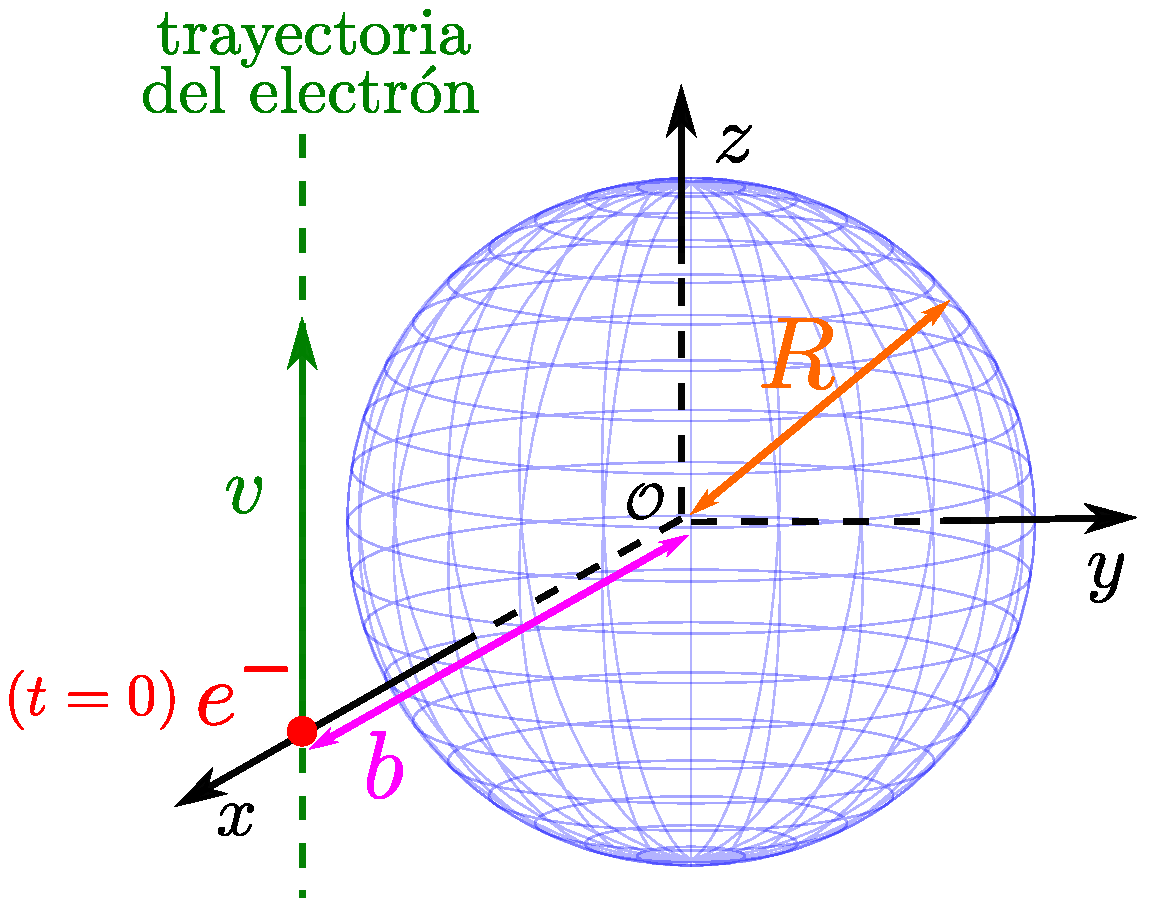
\includegraphics[width=0.5\linewidth]{17-imagenes/3-AppendixB/system_S.pdf}
\caption{\label{fig: system S Surface} Superficie de integración $S$ de radio $R$, junto a la trayectoria del electrón colocada en $\vv{r}=(0,b,vt)$.}
\end{figure}

Para comparar los órdenes de magnitud, se utilizará el valor más pequeño reportado para la TMA ($\Delta L_{\rm min} \sim 10^{-4} \hbar$) \cite{castellanos2021phdthesis, castellanos2021angular,castellanos2023theory}, el cual se usará como referencia en la TMA debida al campo externo calculada en este apéndice. También se compararán los resultados obtenidos con el error numérico de la cuadratura de Gauss-Kronrod \cite{kahaner1989numerical}.

En la Fig. \ref{fig: results ext Delta L}\hyperref[fig: results ext Delta L]{$\mathbf{a)}$} se presenta la TMA en función del orden multipolar $\ell$, manteniendo constante el radio de la NP $a=1$ nm, el parámetro de impacto $b = 5.5$ nm y la rapidez del electrón $v = 0.5\, c$. Los puntos se unen con una línea continua para una mejor visualización. Se observa que la TMA es considerablemente más pequeña que el valor mínimo reportado ($\Delta L_{\rm min} \sim 10^{-4} \hbar$) por $16$ órdenes de magnitud, y que el error numérico es $17$ órdenes de magnitud más pequeño que $\Delta L_{\rm min}$, lo que se equipara a la TMA en este caso. En las subfiguras subsecuentes se consideraron hasta el orden multipolar $\ell=10$ para realizar los cálculos. 

La Fig. \ref{fig: results ext Delta L}\hyperref[fig: results ext Delta L]{$\mathbf{b)}$} muestra la TMA en función de la rapidez del electrón, manteniendo constante el radio de la NP $a=1$ nm y el parámetro de impacto $b = 5.5$ nm. Se puede observar que, para velocidades pequeñas, la TMA crece abruptamente, pero sigue siendo 16 órdenes de magnitud más pequeña que $\Delta L_{\rm min}$ en cualquier velocidad. Además, el error numérico nuevamente está muy cercano al valor de $\Delta L$. En la Fig. \ref{fig: results ext Delta L}\hyperref[fig: results ext Delta L]{$\mathbf{c)}$} se presenta la TMA en función del parámetro de impacto, manteniendo constante el radio de la NP $a=1$ nm y la rapidez del electrón $v = 0.5\, c$. Para parámetros de impacto pequeños, la TMA crece abruptamente, pero sigue siendo 15 órdenes de magnitud más pequeña que $\Delta L_{min}$ sin importar la cercanía del electrón a la NP. También se observa que el error numérico está muy cerca del valor de $\Delta L$. 

Por último, en la Fig. \ref{fig: results ext Delta L}\hyperref[fig: results ext Delta L]{$\mathbf{d)}$} se muestra la TMA en función del radio $R$ de la superficie de integración $S$, manteniendo constante el radio de la NP $a = 1$ nm, el parámetro de impacto $b = 5.5$ nm y la rapidez del electrón $v = 0.5\, c$. Se puede observar que para velocidades pequeñas la TMA crece abruptamente, pero sigue siendo 16 órdenes de magnitud más pequeña que $\Delta L_{min}$ en cualquier velocidad y el error numérico permanece cercano al valor de $\Delta L$.

\begin{figure}[ht!]
\centering
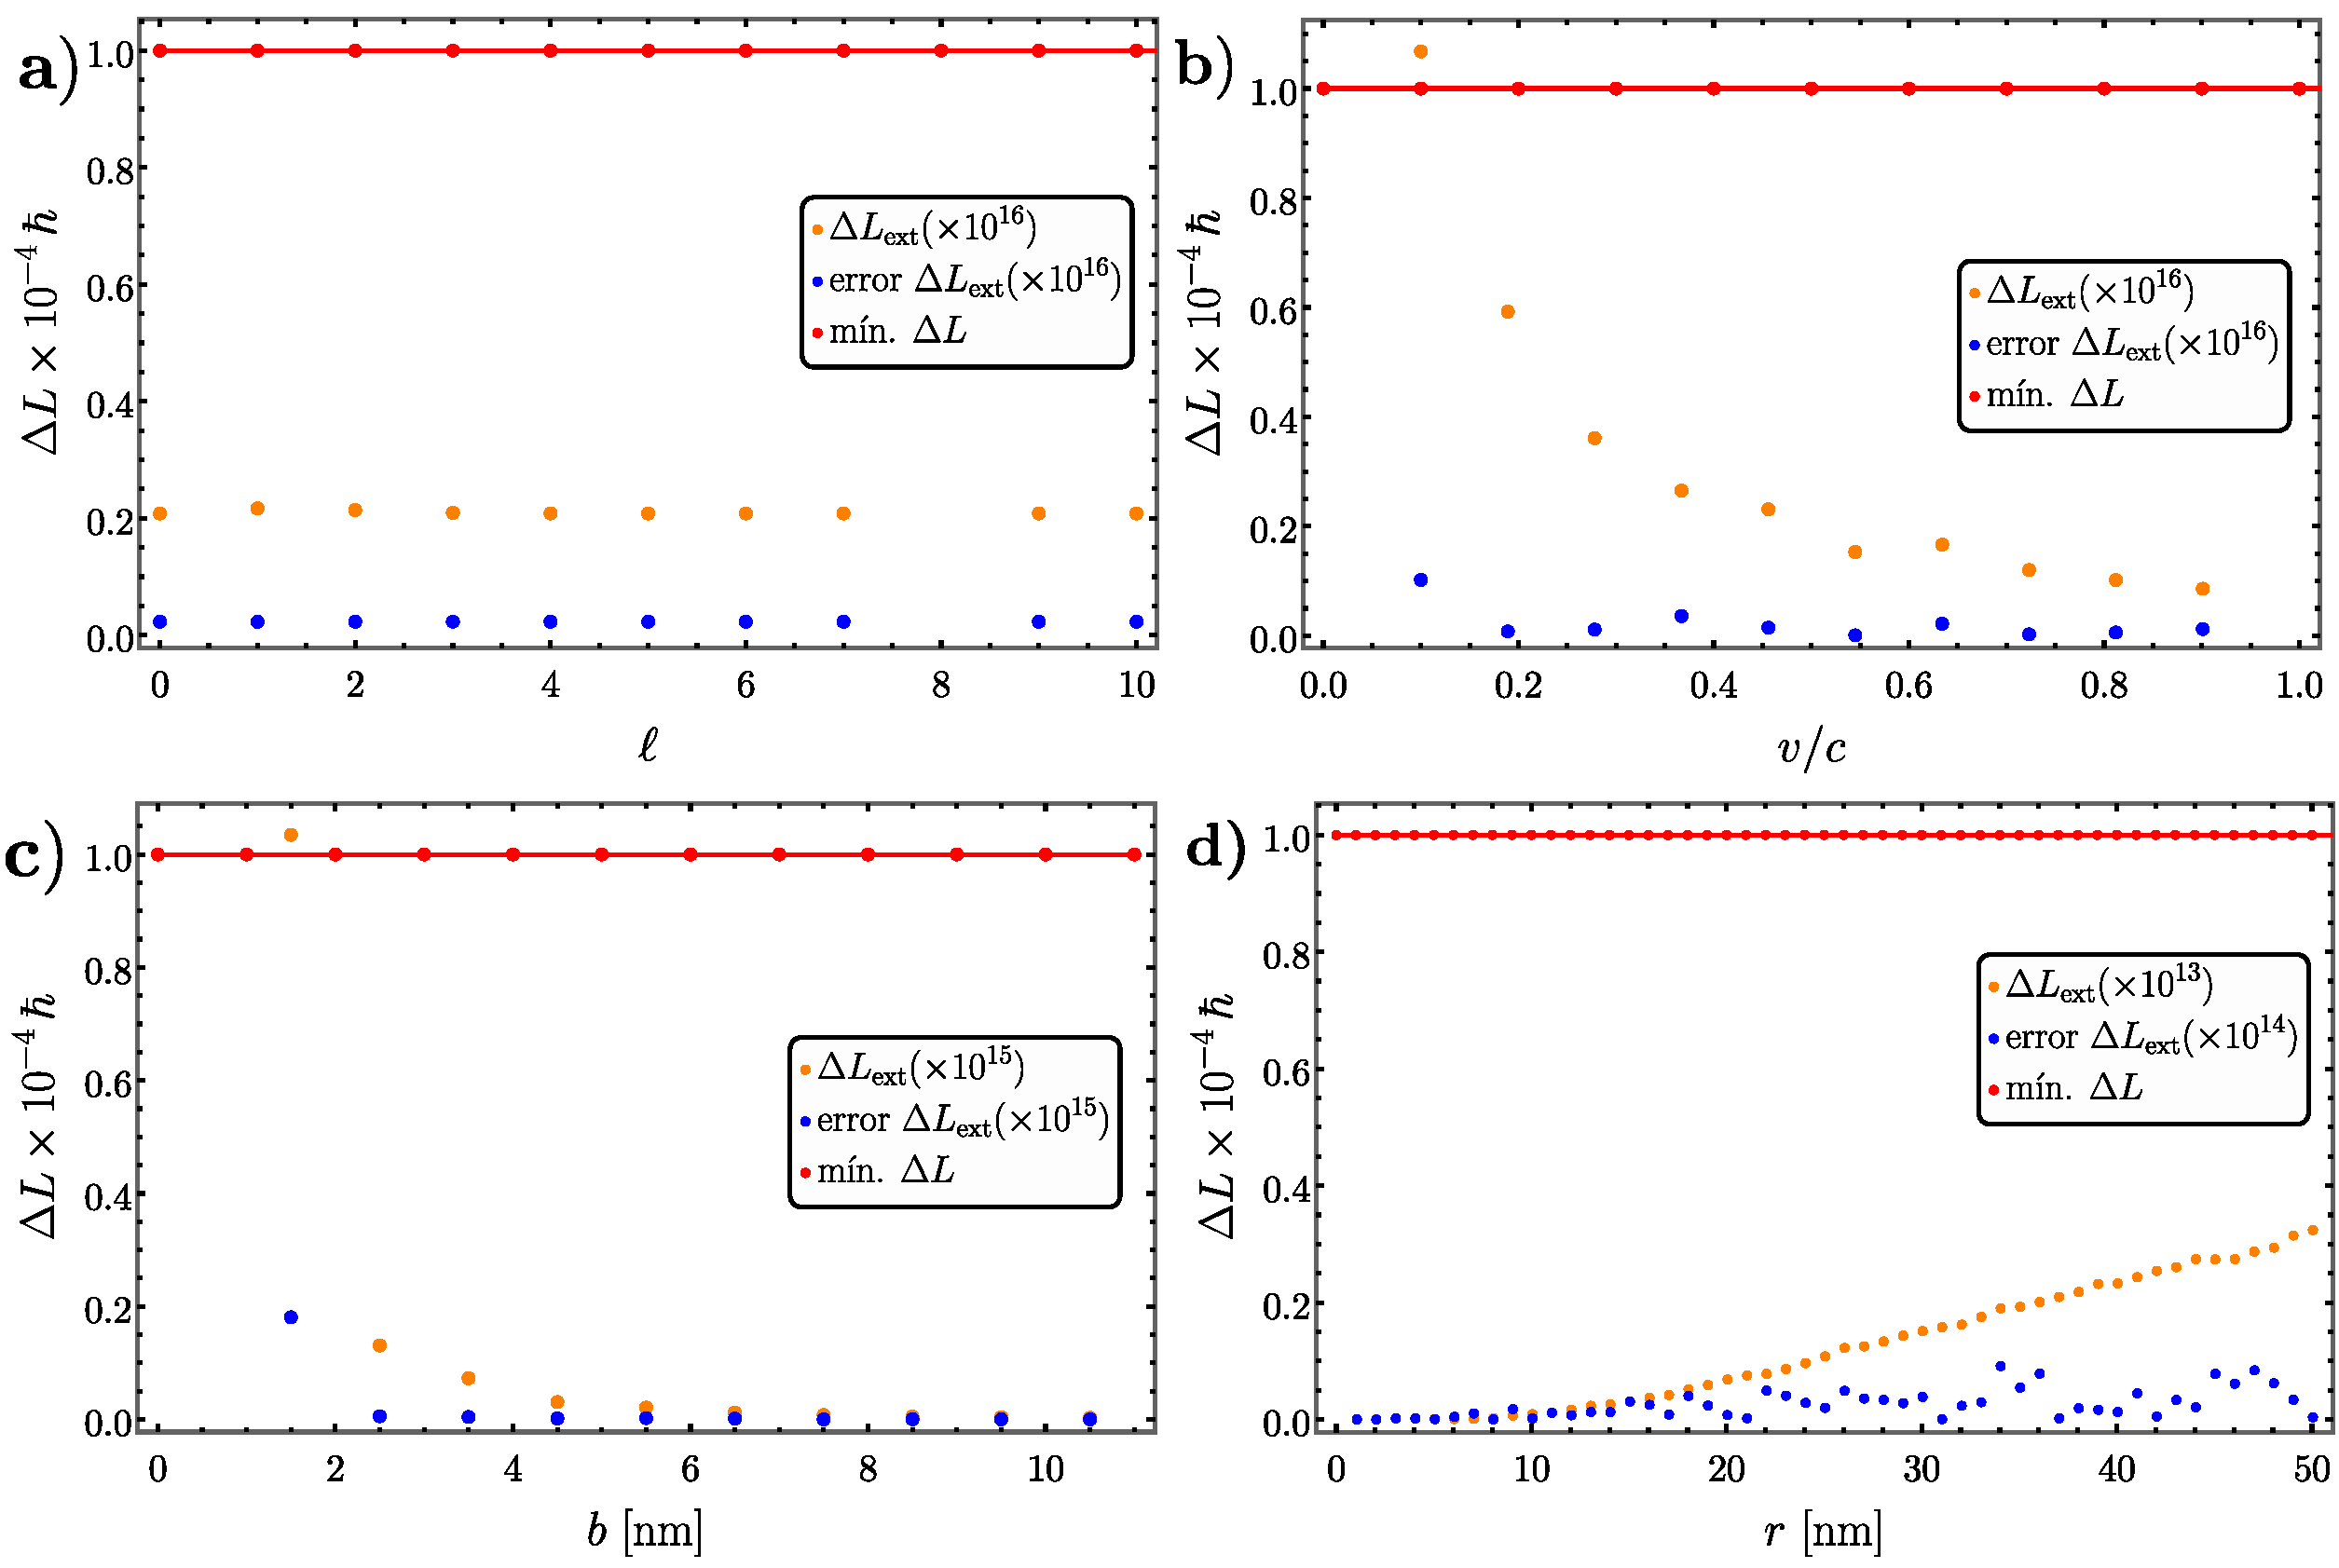
\includegraphics[width=0.8\linewidth]{17-imagenes/3-AppendixB/Results.pdf}
\caption{\label{fig: results ext Delta L} Resultados del cálculo de la transferencia de momento angular, debida al campo externo del electrón, unidos por una línea continua como ayuda visual $\mathbf{a)}$ en función de  el orden multipolar $\ell$, con $a=1$ nm y $b=5.5$ nm; $\mathbf{b)}$ en función de la rapidez del electrón $v$, con $a=1$ nm y $b=5.5$ nm; $\mathbf{c)}$ en función del parámetro de impacto, con $a=1$ nm y $v=0.5 \,c$ nm; y $\mathbf{d)}$ en función del radio $R$ de la superficie de integración $S$, con $a=1$ nm y $b=R +0.45$ nm, donde se ha tenido cuidado de que la superficie de integración no contenga la trayectoria del electrón.}
\end{figure}